% ════════════════════════════════════════════
% 3. 数据理解
% ════════════════════════════════════════════
\section{数据理解}

\subsection{粒度、结构与因果角色}

一行记录对应一条帖子，没有重复行，也没有跨期观测，因此样本是帖级截面数据。缺少发布时间戳并不等于没有时间信息：粉丝规模随月份单调累积，$X_4$ 事实上充当了伪时间轴，这一点在第 4.3 节展开。按发帖前运营人员能否决定划分因果角色，$X_2$ 至 $X_7$ 属于发帖决策变量，$X_1$ 由历史积累决定、属于账号状态变量，$Y_1$ 是发布后的结果。状态变量与决策变量的区别决定了后文的解释口径：决策变量的系数可以读作投放建议，状态变量的系数只能读作账户规模的伴随差异。

表\ref{tab:desc}给出主要变量的量级与离散程度。曝光均值 29,586 次、中位数 9,051 次，均值是中位数的 3.27 倍，最大值 1,110,282 次达到中位数的 122.67 倍，重尾特征明确；粉丝规模均值 123,194 人、标准差 16,273 人，最大值与最小值之比仅 1.71，量级跨度有限，但 500 条帖子只取到 90 个不同数值，说明粉丝数按天或按批次更新、同一数值被多条帖子共享。

{\small
\begin{longtable}{>{\centering\arraybackslash}p{0.080\textwidth}>{\centering\arraybackslash}p{0.080\textwidth}>{\centering\arraybackslash}p{0.140\textwidth}>{\centering\arraybackslash}p{0.120\textwidth}>{\centering\arraybackslash}p{0.120\textwidth}>{\centering\arraybackslash}p{0.110\textwidth}>{\centering\arraybackslash}p{0.130\textwidth}>{\centering\arraybackslash}p{0.100\textwidth}>{\centering\arraybackslash}p{0.100\textwidth}}
  \caption{主要变量的描述统计}
  \label{tab:desc} \\
  \toprule
  变量 & 样本量 & 均值 & 标准差 & 中位数 & 最小值 & 最大值 & 偏度 & 峰度 \\
  \midrule
  \endfirsthead
  \caption{主要变量的描述统计（续）} \\
  \toprule
  变量 & 样本量 & 均值 & 标准差 & 中位数 & 最小值 & 最大值 & 偏度 & 峰度 \\
  \midrule
  \endhead
  \bottomrule
  \endfoot
  X1 & 500 & 123,194 & 16,273 & 129,600 & 81,370 & 139,441 & -0.9795 & -0.2759 \\
  X3 & 500 & 1.88 & 0.8527 & 2 & 1 & 3 & 0.2313 & -1.5836 \\
  X4 & 500 & 7.038 & 3.3079 & 7 & 1 & 12 & -0.1219 & -1.1371 \\
  X5 & 500 & 4.15 & 2.0307 & 4 & 1 & 7 & -0.1022 & -1.2747 \\
  X6 & 500 & 7.84 & 4.3686 & 9 & 1 & 23 & 0.2132 & -0.8252 \\
  X7 & 499 & 0.2786 & 0.4487 & 0 & 0 & 1 & 0.9879 & -1.024 \\
  Y1 & 500 & 29,586 & 76,803 & 9,051 & 570.0 & 1,110,282 & 8.3259 & 93.0526 \\
  logY & 500 & 9.3806 & 1.1781 & 9.1107 & 6.3474 & 13.9201 & 0.7341 & 0.8209 \\
  logX1 & 500 & 11.7118 & 0.1435 & 11.7722 & 11.3068 & 11.8454 & -1.1541 & 0.1845 \\
\end{longtable}
}


\subsection{变量类型与建模角色}

图\ref{fig:dict}把 8 个字段的类型、角色与缺失状态集中呈现：$X_1$ 与 $Y_1$ 为连续变量，$X_2$、$X_3$ 为名义变量，$X_4$ 至 $X_6$ 为周期性时间标记，$X_7$ 为二元指示变量且是唯一存在缺失的字段。周期变量没有天然的等距含义，若按数值直接进入模型会把“12 月与 1 月相邻”误读为“12 月比 1 月大 11 个单位”，因此按类别处理。

\begin{figure}[htbp]
  \centering
  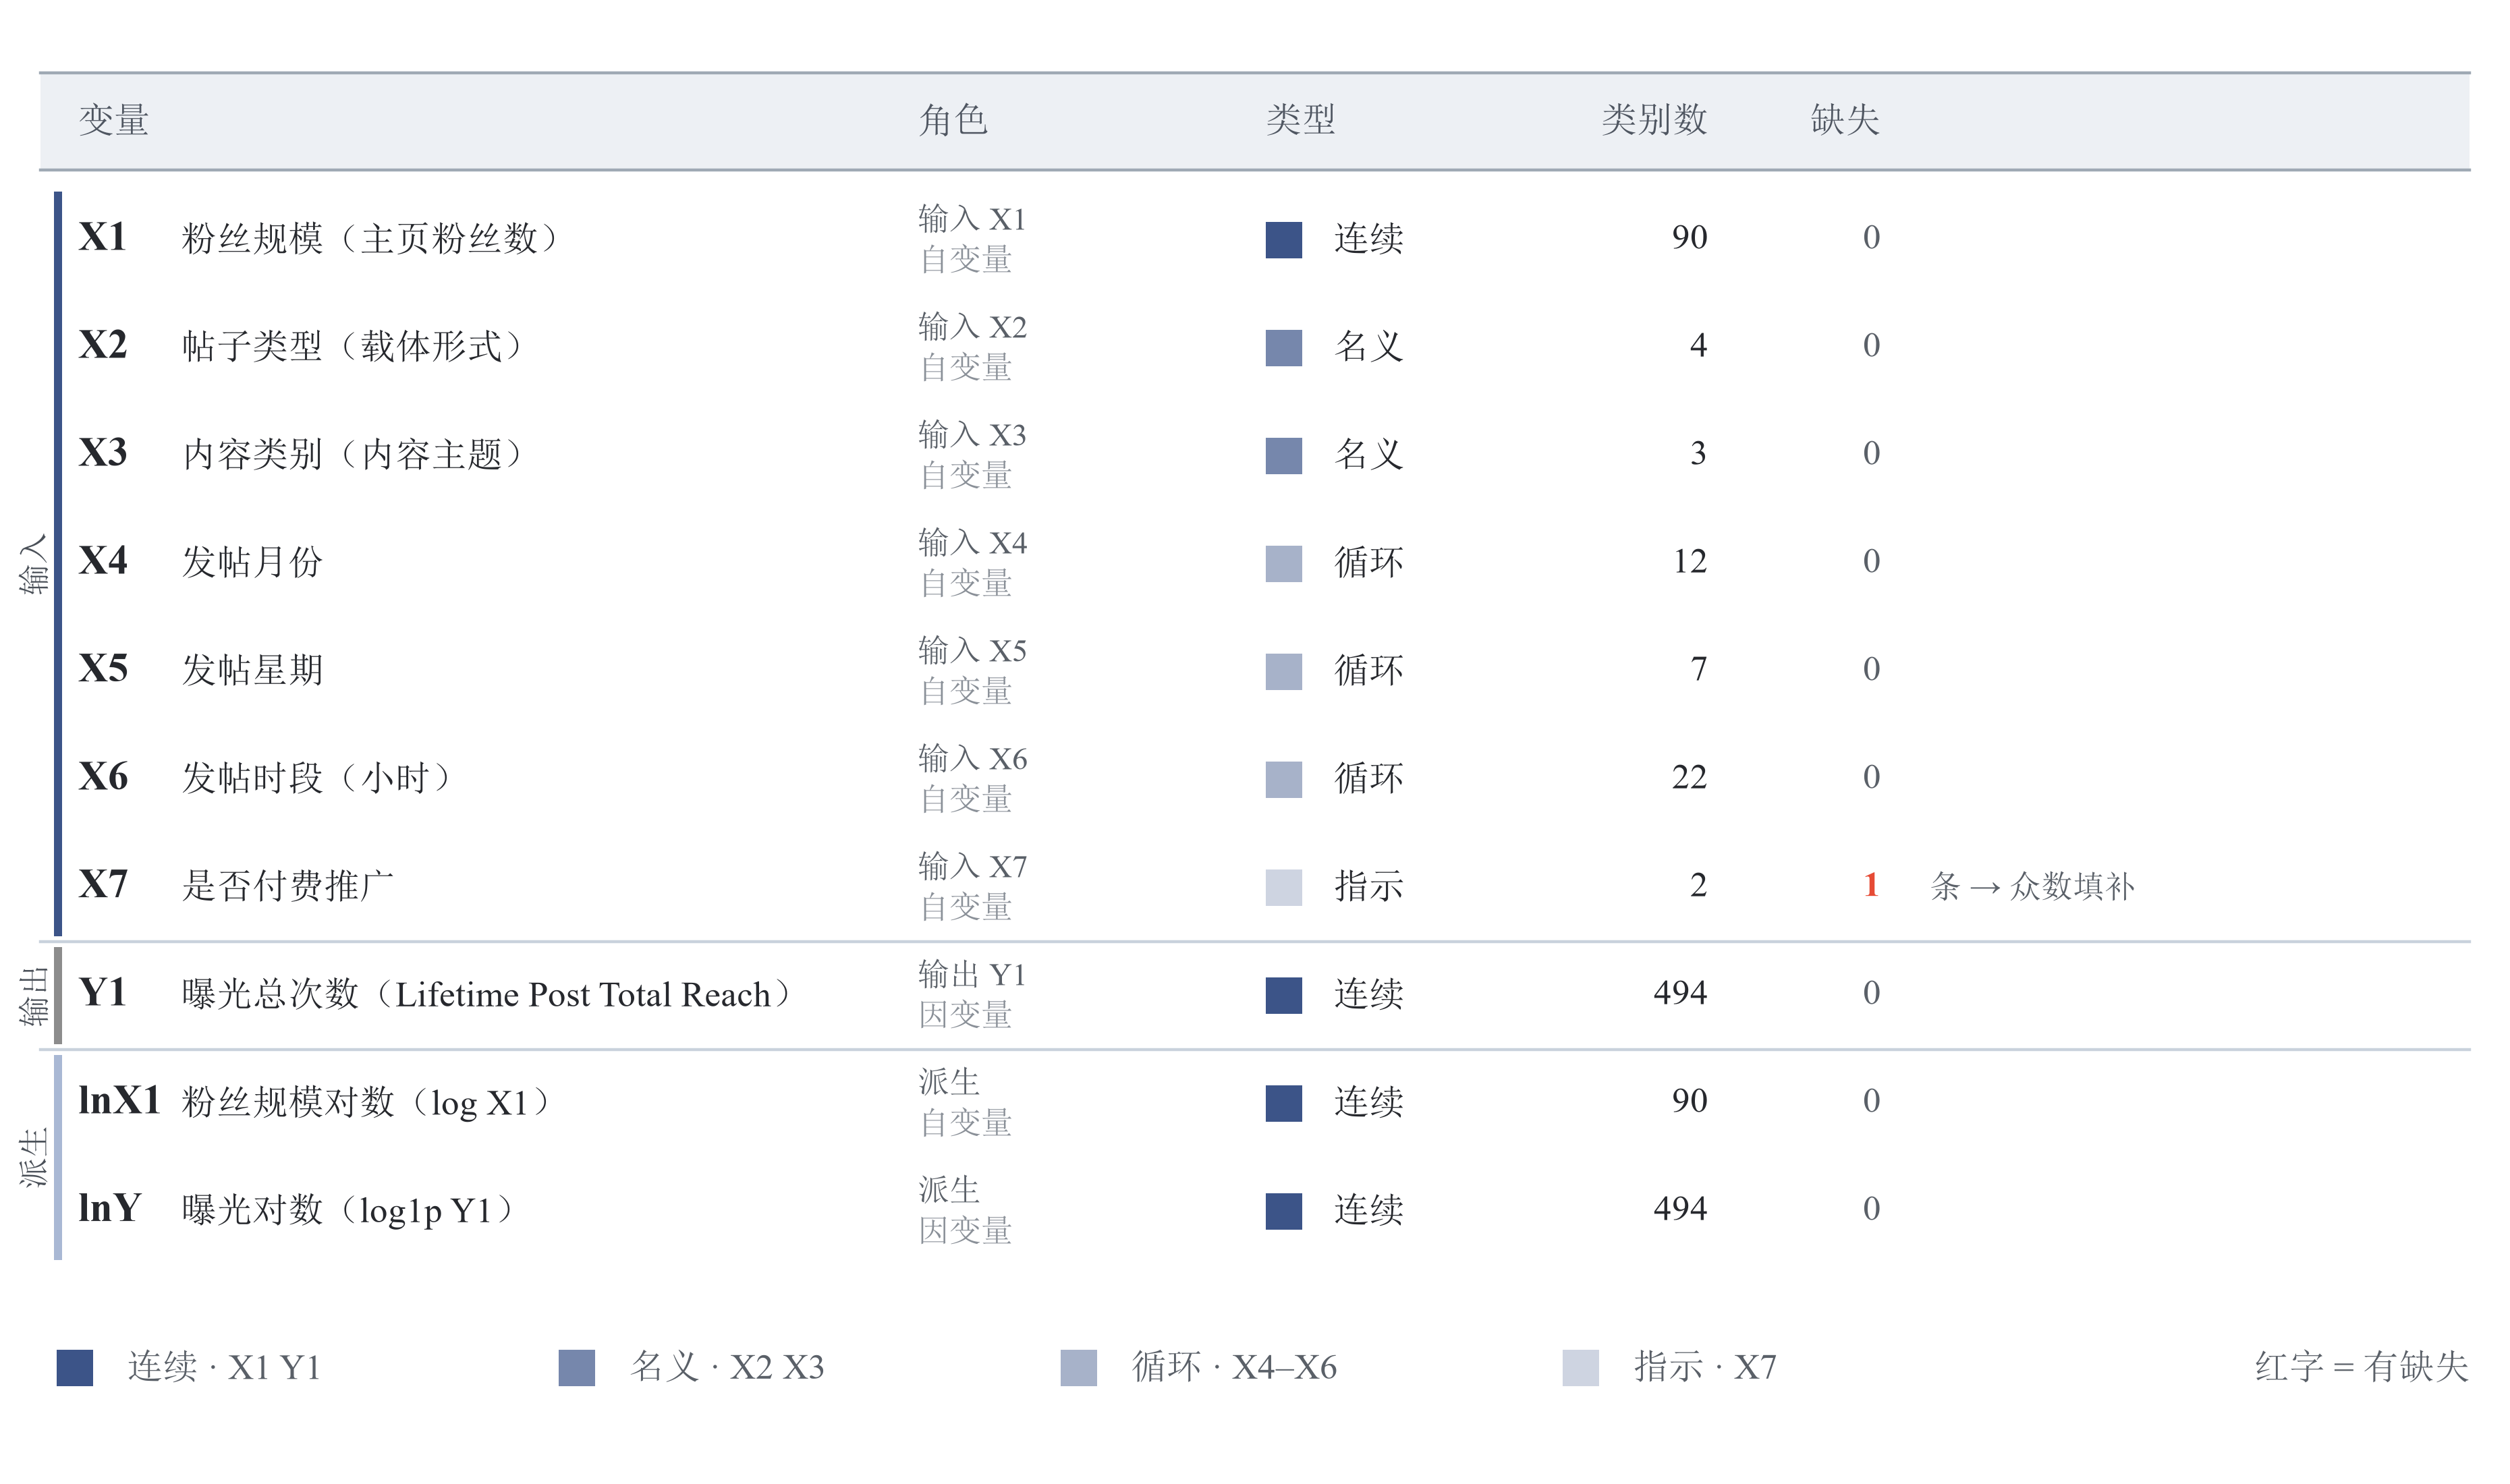
\includegraphics[width=0.62\textwidth]{../求解/问题一/结果/图14_变量字典与缺失.png}
  \caption{变量字典、类型与建模角色}
  \label{fig:dict}
\end{figure}

{\small
\begin{longtable}{>{\centering\arraybackslash}p{0.070\textwidth}>{\centering\arraybackslash}p{0.270\textwidth}>{\centering\arraybackslash}p{0.100\textwidth}>{\centering\arraybackslash}p{0.150\textwidth}>{\centering\arraybackslash}p{0.260\textwidth}>{\centering\arraybackslash}p{0.080\textwidth}}
  \caption{变量字典、类型与建模角色}
  \label{tab:dict} \\
  \toprule
  变量 & 含义 & 数据类型 & 因果角色 & 取值范围/类别 & 缺失数 \\
  \midrule
  \endfirsthead
  \caption{变量字典、类型与建模角色（续）} \\
  \toprule
  变量 & 含义 & 数据类型 & 因果角色 & 取值范围/类别 & 缺失数 \\
  \midrule
  \endhead
  \bottomrule
  \endfoot
  X1 & 粉丝规模（主页粉丝数） & 连续 & 状态/规模 & 81,370–139,441 & 0 \\
  X2 & 帖子类型（载体形式） & 名义 & 发帖决策 & Photo/Status/Link/Video & 0 \\
  X3 & 内容类别（内容主题） & 名义 & 发帖决策 & 1/2/3 & 0 \\
  X4 & 发帖月份 & 有序/周期 & 发帖决策（时机） & 1–12 & 0 \\
  X5 & 发帖星期 & 有序/周期 & 发帖决策（时机） & 1–7 & 0 \\
  X6 & 发帖时段（小时） & 有序/周期 & 发帖决策（时机） & 0–23（样本 1–23） & 0 \\
  X7 & 是否付费推广 & 二元 & 发帖决策 & 0/1 & 1 \\
  Y1 & 曝光总次数（Lifetime Post Total Reach） & 连续（计数） & 结果 & 570–1,110,282 & 0 \\
\end{longtable}
}


\subsection{分布形态与重尾}

曝光量呈典型右偏厚尾，偏度 8.33、峰度 93.05，远超正态分布参考范围；直方图在对数横轴上仍向右拖尾（图\ref{fig:dist}左上）。这种形态下直接对原始曝光建模会让少数百万级帖子主导最小二乘的残差平方和，因此后续以 $\log(1+Y_1)$ 为因变量，系数的含义也随之变为近似的百分比效应。图\ref{fig:dist}其余三个面板给出分组差异：付费组中位曝光 12,060 次、自然组 8,443 次，中位数提升 42.8\%；视频组中位数最高（56,950 次），但仅 7 条；三类主题的中位数分别为 10,417、8,962 与 8,303 次。分组差异为后续回归提供线索，但在未控制月份与内容构成前不能当作净效应。

\begin{figure}[htbp]
  \centering
  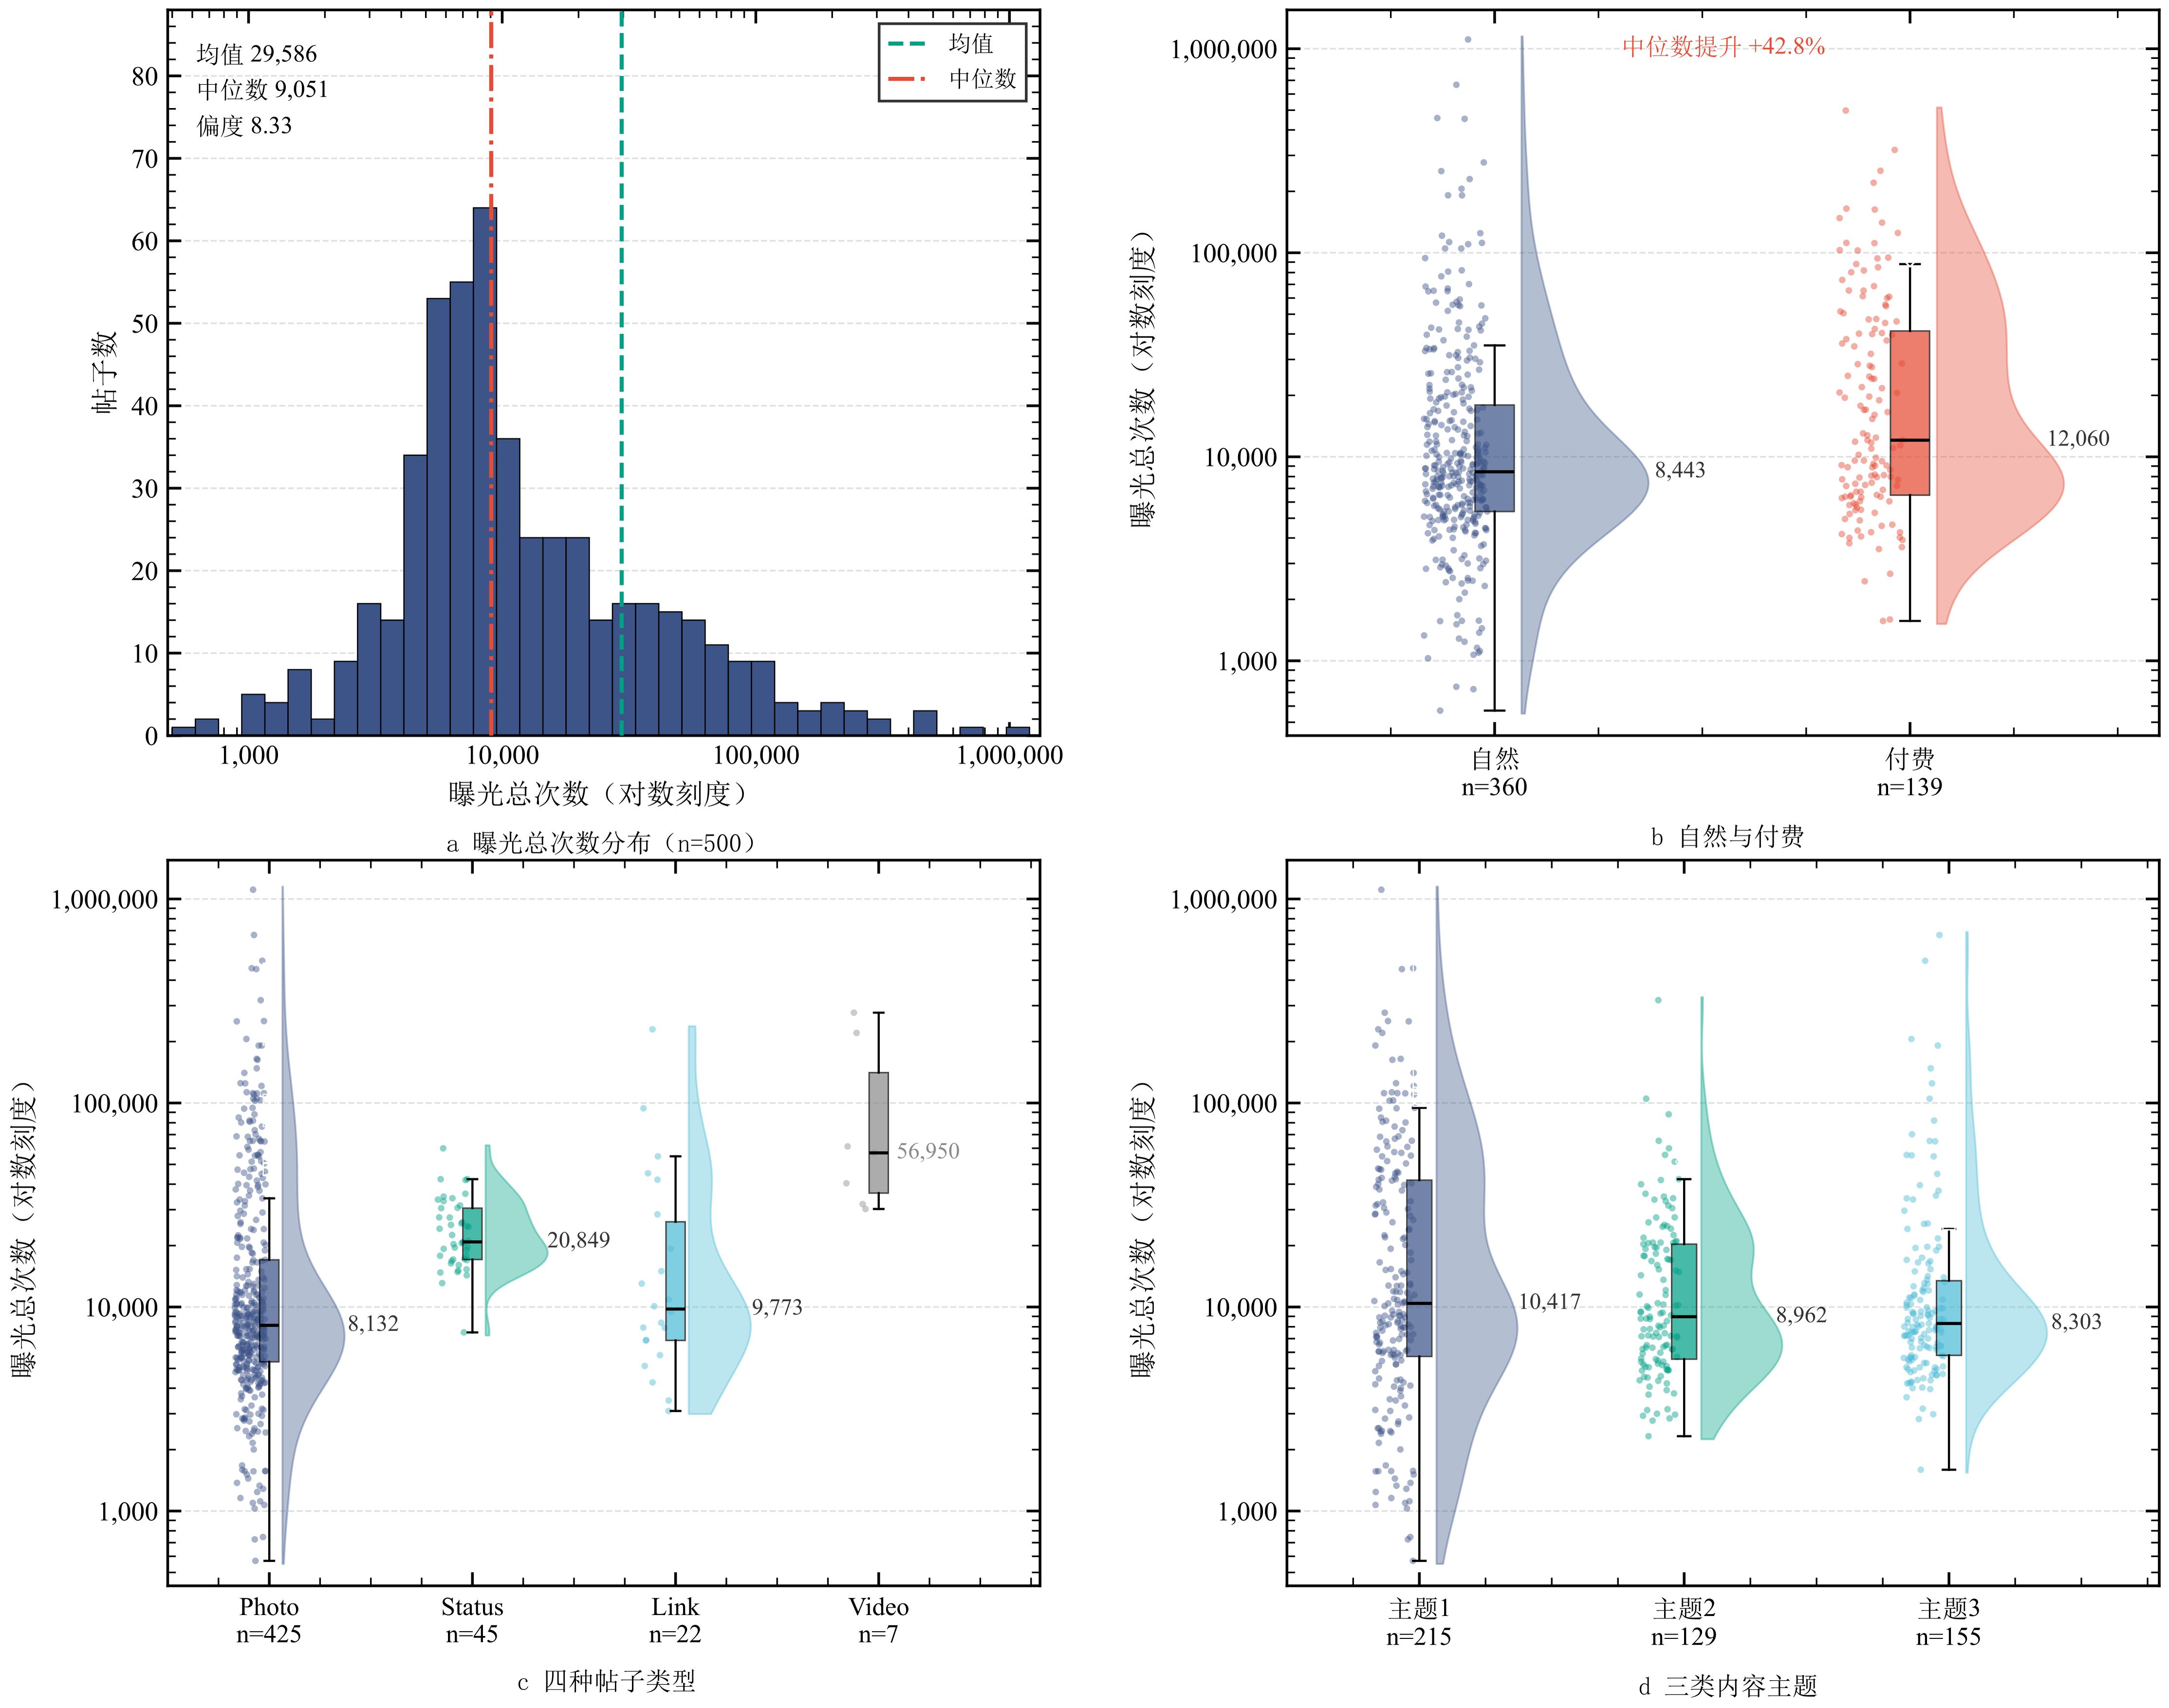
\includegraphics[width=0.60\textwidth]{../求解/问题一/结果/图1_曝光与分组分布.png}
  \caption{曝光量分布与分组差异：对数直方图与三组雨云图}
  \label{fig:dist}
\end{figure}
